% nladoc.tex V2.0, 13 May 2010

\documentclass[times]{nlaauth}

\usepackage{moreverb}

\usepackage[colorlinks,bookmarksopen,bookmarksnumbered,citecolor=red,urlcolor=red]{hyperref}
\usepackage{tikz}
\usetikzlibrary{shapes,arrows,trees,snakes,decorations.pathreplacing,fit}
\usepackage{tkz-euclide}
\usepackage{pgfplots}
\usetkzobj{all} 

\definecolor{utorange}{RGB}{203,96,21}
\definecolor{utblack}{RGB}{99,102,106}
\definecolor{utbrown}{RGB}{110,98,89}
\definecolor{utsecbrown}{RGB}{217,200,158}
\definecolor{utsecgreen}{RGB}{208,222,187}
\definecolor{utsecblue}{RGB}{127,169,174}


\newcommand{\gsnote}[1]{\textcolor{blue}{GS: #1}}


\newcommand\BibTeX{{\rmfamily B\kern-.05em \textsc{i\kern-.025em b}\kern-.08em
T\kern-.1667em\lower.7ex\hbox{E}\kern-.125emX}}

\def\volumeyear{2013}

\begin{document}

\runningheads{Sundar~et~al.}{High-order Geometric Multigrid}

\title{On Geometric Multigrid Algorithms for High-order Finite Element Discretizations}

\author{Hari Sundar\corrauth, Georg Stadler, Omar Ghattas and George Biros}

\address{Institute for Computational Engineering \& Sciences, University of Texas, Austin, TX 78712}

\corraddr{\texttt{hari@ices.utexas.edu}}

\begin{abstract}
\input {homg_abstract.tex}
\end{abstract}

\keywords{geometric multigrid, high-order discretizations, p-multigrid}

\maketitle


\section{Introduction}

%We are interested on asymptotically
%optimal---$\mathcal{O}(N)$---complexity solvers for approximating the
%solution of elliptic partial differential equations (PDEs), where $N$
%is the number of unknowns.  Multigrid is such a solver. In practice
%however, multigrid performs best for low-order uniform discretizations
%with smooth coefficients. 

We target parallel geometric multigrid methods for solving systems
arising from higher order (we target polynomial orders up to 8)
discretizations of elliptic partial differential equations. In
particular, our interest is on large-scale problems with complex
geometry and adaptively refined meshes, and the implementation of
these methods on parallel high performance computing platforms. Thus,
we favor (1) matrix-free methods, i.e., method that do not require
assembled finite element matrices, (2) methods that can be
parallelized on shared or distributed memory architectures, and (3)
cache-efficient methods with dominantly local memory access.

High order spatial discretizations can have significant advantages
over low order methods, especially when the solution is smooth and
high accuracy is desired. However, the sparsity of finite element (or
finite difference) operators decreases as the polynomial approximation
order increases, which makes the application of high order operators
to vectors computationally significantly more expensive. This is also
true if matrix-free methods are used, i.e., system matrices are never
assembled, but their application on vectors is implemented through
elemental loops.  Besides the loss of sparsity, another challenge in
high-order discretizations is due to that fact that the discretization
matrices loose useful structural properties, such as the M-matrix
property that allows to prove convergence of iterative solvers such as
the Jacobi or Gauss-Seidel method.

\gsnote{Needs a literature review.}

%High-order discretizations offer several advantages.  According to
%standard isoparametric polynomial approximation theory,
%% the approximation error in the $L_2$-norm is bounded by,
%% \[
%% \|u-u_h\|_{L_2} \le Ch^{p+1}\|u\|_{H^{p+1}(\Omega)},
%% \]   
%% where $\|\cdot\|_{H^p}$ is the standard $H^p$ Sobolev norm, $\|\cdot\|_{L_2}$ is the $L_2$-norm, $u$ is the exact solution of the PDE, and $u_h$ is the solution of the $h$-discrete problem. Therefore, 
%by using a finite element basis of at least degree $p$, we can achieve
%very fast $\mathcal{O}(N^{-(p+1)})$ convergence for sufficiently
%smooth problems while improving the locality and thus the CPU
%efficiency of the calculations.


Although there are examples of using Algebraic Multigrid directly on
operators resulting from higher-order discretizations, limited work
has been done on using geometric multigrid with higher-order
discretizations. To the best of our knowledge, no prior work on using
geometric multigrid for solving systems arising from higher-order
discretizations on arbitrary geometries using highly adapted meshes.



%In this work, we develop
%geometric multigrid methods to support higher-order discretizations
%($1\le p\le 8$) and compare  against preconditioning using the
%co-located linear operator.

% We evaluate using variable-coefficient
%Poisson problems on $2D$ and $3D$ domains. We demonstrate that by
%using appropriate inter-grid transfer operators and smoothers,
%mesh-independent convergence is possible ($1\le p\le8$) for the {\em
%direct} approach. For the direct approach, best results are obtained
%using the symmetric successive over-relaxation (SSOR) smoother. We
%conclude with thoughts on the parallelization of the proposed
%approach.\\[2ex]


\gsnote{Unify notion of mesh/grid etc}



\section{Meshing, High-order FEM}

 Our method is designed for meshes that are built from an unstructured
hexahedral macro mesh, in which each macro element is adaptively
refined as an octree. This forest-of-octrees approach enables us to
generate meshes for complex geometries with arbitrary levels of local
refinement. We use geometric multigrid (GMG) for each of the octrees
and algebraic multigrid (AMG) as the coarse grid solver. We designed
our GMG sweeps to entirely avoid collectives, thus minimizing
communication cost. Recently \cite{SundarBirosBursteddeEtAl12}, we
presented weak and strong scaling results for the 3D
variable-coefficient Poisson problem using linear discretization that
demonstrate high parallel scalability. Here we explore various
approaches for extending our geometric multigrid solver to support
higher-order discretizations.

For three-dimensional hexahedral mesh finite element discretizations
with polynomial degree $p$, element matrices are of size
$n=(p+1)^3$. The naive assembly and application of these elemental
matrices requires $\mathcal O(p^9)$ operatrions, but exploiting the
tensor structure of the basis functions allows to reduce this to
$\mathcal O(p^7)$ operations.


\section{Approaches for High-order Multigrid}

% talk about the 4 main approaches and prior work.

In this section, we summarize different approaches for geometric
multigrid-based solvers and preconditioners for higher-order
finite-element discretizations. These methods can also be
appropriately combined.

\subsection{High-order $h$-multigrid}\label{subsec:h}
A direct generalization of geometric multigrid from first order to
higher order discretizations is to use high order restriction and
prolongation operators together with the linear systems that result
from the higher-order discretizations on each coarse level.  The main
difficulty in this approach is that it requires smoothers for high
order systems matrices, which usually have less favorable properties
compared to their low order counterparts; For instance, higher-order
discretizations of scalar elliptic operators are usually not
M-matrices, which is a useful property to prove the convergence of
smoothers such as Jacobi of Gauss-Seidel.

\begin{figure}
		% illustration for p-multigrid
		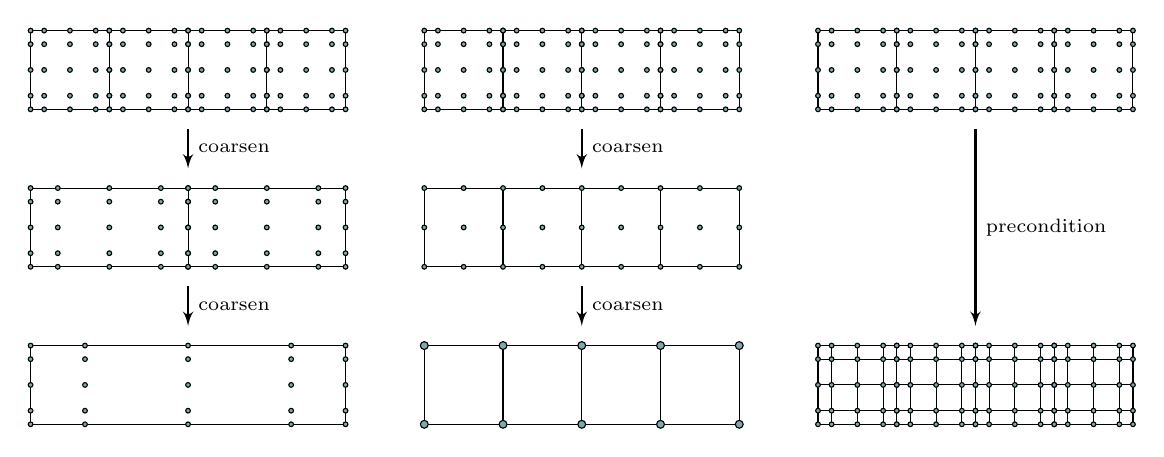
\begin{tikzpicture}
	
		% homg
		\draw (-5,4) grid +(4,1);
		\foreach \e in {-5,...,-2}
		\foreach \x in {0,0.1727,0.5,0.8273, 1.0} {
			\draw[fill=utsecblue] (\e+\x, 4) circle (0.03);
			\draw[fill=utsecblue] (\e+\x, 4.1727) circle (0.03);
			\draw[fill=utsecblue] (\e+\x, 4.5) circle (0.03);
			\draw[fill=utsecblue] (\e+\x, 4.8273) circle (0.03);
			\draw[fill=utsecblue] (\e+\x, 5) circle (0.03);
		}
		%\node at (5,4.5) {\small $p=4$};
	
		\draw[-latex',thick] (-3, 3.75) -- node[right] {{\scriptsize coarsen}} (-3, 3.25);
	
		\draw (-5,2) rectangle +(4,1);
		\draw (-3,2) -- (-3,3);
		
		\foreach \e in {-5,-3}
		\foreach \x in {0,0.1727,0.5,0.8273, 1.0} {
			\draw[fill=utsecblue] (\e+2*\x, 2) circle (0.03);
			\draw[fill=utsecblue] (\e+2*\x, 2.1727) circle (0.03);
			\draw[fill=utsecblue] (\e+2*\x, 2.5) circle (0.03);
			\draw[fill=utsecblue] (\e+2*\x, 2.8273) circle (0.03);
			\draw[fill=utsecblue] (\e+2*\x, 3) circle (0.03);
		}
		%\node at (5,2.5) {\small $p=2$};
	
		\draw[-latex',thick] (-3, 1.75) -- node[right] {{\scriptsize coarsen}} (-3, 1.25);
	
		\draw (-5,0) rectangle +(4,1);
		\foreach \x in {0,0.1727,0.5,0.8273, 1.0} {
			\draw[fill=utsecblue] (-5+4*\x, 0) circle (0.03);
			\draw[fill=utsecblue] (-5+4*\x, 0.1727) circle (0.03);
			\draw[fill=utsecblue] (-5+4*\x, 0.5) circle (0.03);
			\draw[fill=utsecblue] (-5+4*\x, 0.8273) circle (0.03);
			\draw[fill=utsecblue] (-5+4*\x, 1) circle (0.03);
		}
		
	%% p-multigrid
		\draw (0,4) grid +(4,1);
		\foreach \e in {0,...,3}
		\foreach \x in {0,0.1727,0.5,0.8273, 1.0} {
			\draw[fill=utsecblue] (\e+\x, 4) circle (0.03);
			\draw[fill=utsecblue] (\e+\x, 4.1727) circle (0.03);
			\draw[fill=utsecblue] (\e+\x, 4.5) circle (0.03);
			\draw[fill=utsecblue] (\e+\x, 4.8273) circle (0.03);
			\draw[fill=utsecblue] (\e+\x, 5) circle (0.03);
		}
		%\node at (5,4.5) {\small $p=4$};
	
		\draw[-latex',thick] (2, 3.75) -- node[right] {{\scriptsize coarsen}} (2, 3.25);
	
		\draw (0,2) grid +(4,1);
		\foreach \x in {0,0.5,...,4} {
			\draw[fill=utsecblue] (\x, 2) circle (0.03);
			\draw[fill=utsecblue] (\x, 2.5) circle (0.03);
			\draw[fill=utsecblue] (\x, 3) circle (0.03);
		}
		%\node at (5,2.5) {\small $p=2$};
	
		\draw[-latex',thick] (2, 1.75) -- node[right] {{\scriptsize coarsen}} (2, 1.25);
	
		\draw (0,0) grid +(4,1);
		\foreach \x in {0,1,2,3,4} {
			\draw[fill=utsecblue] (\x, 0) circle (0.05);
			\draw[fill=utsecblue] (\x, 1) circle (0.05);
		}
		%\node at (5,0.5) {\small $p=1$};
		
		%% collocated
			\draw (5,4) grid +(4,1);
			\foreach \e in {5,...,8}
			\foreach \x in {0,0.1727,0.5,0.8273, 1.0} {
				\draw[fill=utsecblue] (\e+\x, 4) circle (0.03);
				\draw[fill=utsecblue] (\e+\x, 4.1727) circle (0.03);
				\draw[fill=utsecblue] (\e+\x, 4.5) circle (0.03);
				\draw[fill=utsecblue] (\e+\x, 4.8273) circle (0.03);
				\draw[fill=utsecblue] (\e+\x, 5) circle (0.03);
			}
			%\node at (2, 1.8) {\tiny $p=4$};
	
			\draw[-latex',thick] (7, 3.75) -- node[right] {{\scriptsize precondition}} (7, 1.25);
	
			\draw[step=0.5] (4.99,0) grid +(4.01,1);
			\draw (5,0.1727) -- (9,0.1727);
			\draw (5,0.8273) -- (9,0.8273);
			\foreach \e in {5,...,8} {
				\draw (\e+0.1727,0) -- (\e+0.1727,1);
				\draw (\e+0.8273,0) -- (\e+0.8273,1);
				\foreach \x in {0,0.1727,0.5,0.8273, 1.0} {
					\draw[fill=utsecblue] (\e+\x, 0) circle (0.03);
					\draw[fill=utsecblue] (\e+\x, 0.1727) circle (0.03);
					\draw[fill=utsecblue] (\e+\x, 0.5) circle (0.03);
					\draw[fill=utsecblue] (\e+\x, 0.8273) circle (0.03);
					\draw[fill=utsecblue] (\e+\x, 1) circle (0.03);
				}
			}
			% \node at (2, -0.2) {\tiny $p=1$ collocated with $p=4$};
		
		
		
		
		\end{tikzpicture}
		\caption{\label{fig:approaches} Different approaches for high-order multigrid.}
\end{figure}


% This
%approach is more difficult to implement and the cost per iteration
%increases. However, our preliminary results suggest that such an
%approach is the most general.

\subsection{$p$-multigrid}\label{subsec:p}
In the $p$-multigrid approach to high order multigrid, one (initially)
does not coarsen the mesh geometrically, but coarsens the system by
reducing the polynomial order. Starting from an order-$p$ polynomial
basis, the coarser grids correspond to polynomials of order $p/2,
p/4,\ldots,1$, followed by geometric coarsening of the $p=1$ grid
(i.e., the usual low order geometric multigrid). Decreasing the
polynomial order is rather simple and element-local. The latter is
particularly simple for discretizations with nonconforming
meshes. \gsnote{Is that actually true?}. Devising appropriate
smoothers is a challenge for $p$-multigrid.  Moreover, one often finds
dependence of the convergence factor on the order of the polynomial
basis. \gsnote{We need a citation here.}

\subsection{Preconditioning by lower-order operator}\label{subsec:low}
This approach preconditions the higher-order operator by a low order
operator obtained by overlaying the higher-order nodes with a
lower-order (typically linear) finite element mesh. Standard multigrid
is then used for the low order operator, which has more favorable
sparsity properties and thus allows for standard smoothers.  The
construction of a low-order preconditioner based on the nodes of the
high order discretization is a relatively popular approach
\cite{Brown10,Kim07,DevilleMund?}. The resulting method nearly
independent of $p$, and is relatively straightforward to parallelize.
In addition, due to the sparsity of the low order operators,
performing multigrid cycles is faster compared to high order multigrid
(see Section~\ref{subsec:h} above).  However, this speedup does not
come into play on the finest mesh level where the high-order residual
must be computed. Thus, the speedup for a full multigrid cycle when
using the low order operator is limited.  This low-order
preconditioning is not work optimal and the convergence factors can be
lower than when multigrid is applied directly to the higher-order
operator. Also, for nonconforming meshes, constructing the low order
operator can be technical at edges and faces of different size; while
the basis functions for the high order operators can be made
continuous through the use of algebraic constraints at nonconforming
faces, the corresponding low order discretization has discontinuities
at nonconforming faces.

%The advantages of doing
%this are mainly in the simplicity of the approach and the availability
%of parallel multigrid solvers capable of solving such lower-order
%operators.
% The sparsity of the lower-order operators also permits the
%use of AMG for solving the lower-order operators, possibly obtained
%via discretizations on unstructured meshes.

\subsection{Schwarz-based methods}\label{subsec:schwarz}
Another common approach for solving systems arising from higher-order
discretizations is based on local block solves.  The main challenge
with these approaches is that they require solving dense local blocks
either using direct methods or approximations that allow for fast
iterative solution \cite{LottesFischer05,FischerLottes05}. These
methods have been used successfully for spectral element
discretizations with orders significantly larger than 8. However, the
coarse-grid solves can become fairly expensive and is not
straightforward to achieve good parallel scalability. \gsnote{Why?}


\section{Smoothers}
% Chebyshef, Jacobi, SSOR



\section{Performance Model}

talk about a performance model, so we can analyse the various approaches.

\section{Evaluation}

Present results here and analyze based on performance model.



\begin{table}
  \caption{\label{tab:homg} Number of CG iterations/v-cycles to converge to a relative tolerance of $10^{-8}$ for $h$-Multigrid applied to high-order operators on a rectangular domain. A total of 3 grids were used, the finest grid was $32\times 32$, and the coarsest was $8\times 8$.}
		\centering
    \begin{tabular}{|l|c|c|c|c|c|c|} 
	    \hline
				    & \multicolumn{3}{c|}{Multigrid} & \multicolumn{3}{c|}{MG pCG}\\  \cline{2-7}
			order & \scriptsize Jacobi(3)  &\scriptsize  Chebyshev(3)  &\scriptsize SSOR(2) &\scriptsize Jacobi(3)  &\scriptsize  Chebyshev(3)  &\scriptsize SSOR(2) \\
			\hline
				1 & 6 &  5 & 4  &  4  & 4  & 4 \\ 
	    	2 & 7 &  9 & 4  &  5  & 6  & 4 \\
				3 & 8 & 22 & 5  &  6  & 10 & 4 \\
				4 & - & 48 & 8  & 43  & 15 & 6 \\
				5 & - & 150 & 12 & 295 & 27 & 8 \\
				6 & - & - & 27  & - & 51 & 12 \\
				7 & - & - & 81 & - & 105 & 21 \\
				8 & - & - & 298 & - & 204 & 39 \\
			\hline
	  \end{tabular}
\end{table}

\begin{table}
  \caption{\label{tab:hpmg} Number of CG iterations/v-cycles to converge to a relative tolerance of $10^{-8}$ for $hp$-Multigrid applied to high-order operators on a rectangular domain. Starting with a $32\times 32$ high-order grid, we first coarsen in $p$ till $p=1$, and then coarsen in $h$. The coarsest grid in all cases is a $8\times 8$ grid with $p=1$}
		\centering
		\begin{tabular}{|l|c|c|c|c|c|c|} 
	    \hline
				    & \multicolumn{3}{c|}{Multigrid} & \multicolumn{3}{c|}{MG pCG}\\  \cline{2-7}
			order & \scriptsize Jacobi(3)  &\scriptsize  Chebyshev(3)  &\scriptsize SSOR(2) &\scriptsize Jacobi(3)  &\scriptsize  Chebyshev(3)  &\scriptsize SSOR(2) \\
			\hline
				1 & 6  &  5 &  4 & 4 & 4 & 4 \\ 
	    	2 & 7 & 9  & 4 & 5 & 6 & 4 \\
				%3 & 8 & 24 & 5 & 6 & 11 & 4 \\
				4 & - & 46 & 7 & 39 & 15 & 5 \\
				%5 & - & 178 & 13 & - & 28 & 8 \\
				%6 & - & - & 24 & - & 51 & 12 \\
				%7 & - & - & 70 & - & 105 & 19 \\
				8 & - & - & 267 & - & 182 & 36 \\
			\hline
	  \end{tabular}
\end{table}


\begin{table}
  \caption{\label{tab:homg} Number of CG iterations/v-cycles to converge to a relative tolerance of $10^{-8}$ for $h$-Multigrid applied to high-order operators on a fan domain. A total of 3 grids were used, the finest grid was $48\times 16$, and the coarsest was $12\times 4$.}
		\centering
    \begin{tabular}{|l|c|c|c|c|c|c|} 
	    \hline
				    & \multicolumn{3}{c|}{Multigrid} & \multicolumn{3}{c|}{MG pCG}\\  \cline{2-7}
			order & \scriptsize Jacobi(3)  &\scriptsize  Chebyshev(3)  &\scriptsize SSOR(2) &\scriptsize Jacobi(3)  &\scriptsize  Chebyshev(3)  &\scriptsize SSOR(2) \\
			\hline
      1 & 7  & 8  & 4 & 5 & 6 & 4 \\ 
	    2 & 9  & 12 & 5 & 6 & 7 & 4 \\	
			3 & 10 & 26 & 5 & 7 & 12 & 4 \\
      4 & -  & 54 & 8 & 136 & 17 & 6 \\
      5 & - & 171 & 14 & - & 31 & 8 \\
      6 & - & - & 42 & - & 53 & 15 \\
      7 & - & - & 146 & - & 109 & 29 \\
      8 & - & - & 350 & - & -  & 63 \\
      \hline
	  \end{tabular}
\end{table}


\begin{table}
  \caption{\label{tab:hpmg} Number of CG iterations/v-cycles to converge to a relative tolerance of $10^{-8}$ for $hp$-Multigrid applied to high-order operators on a fan domain. Starting with a $48\times 16$ high-order grid, we first coarsen in $p$ till $p=1$, and then coarsen in $h$. The coarsest grid in all cases is a $12\times 4$ grid with $p=1$}
		\centering
		\begin{tabular}{|l|c|c|c|c|c|c|} 
	    \hline
				    & \multicolumn{3}{c|}{Multigrid} & \multicolumn{3}{c|}{MG pCG}\\  \cline{2-7}
			order & \scriptsize Jacobi(3)  &\scriptsize  Chebyshev(3)  &\scriptsize SSOR(2) &\scriptsize Jacobi(3)  &\scriptsize  Chebyshev(3)  &\scriptsize SSOR(2) \\
			\hline
				1 & 6  &  5 &  4 & 4 & 4 & 4 \\ 
        2 & 9 & 12 & 5 & 6 & 8 & 4 \\
				4 & - & 53 & 7 & 100 & 16 & 6 \\
        8 & - & -  & - & - & 200 & 60 \\
			\hline
	  \end{tabular}
\end{table}



\section{Discussion and conclusions}

%Finalize and discuss ramifications.

\begin{itemize}
\item Using multigrid with Jacobi and Jacobi-based Chebyshev smoothing
  as solver either fails to converge or converges slowly at orders
  $p\ge 4$.
\item Using Jacobi-based multigrid as preconditioner in the conjugate
  gradient method, the number of iterations for polynomial orders
  $p=2,3$ is similar to the number of iterations for linear elements.
  In general, for the same number of unknowns one can expect better
  accuracy for higher polynomial order. This advantage has to be
  contrasted with the fact that higher order operators are less sparse
  and thus their application to vectors is more time consuming.  Using
  Jacobi-based smoothers is attractive from a parallel perspective
  since no coloring of unknowns as in SSOR is necessary.
\item Both, high-order $h$-multigrid as well as $p$-multigrid yield
  significantly faster convergence in terms of the number of
  iterations than preconditioning with the low-order
  operator. Although the low order operators are sparser and thus
  faster to apply, the larger number of iterations results in larger
  time-to-solution.
\item Simple problems Chebyshev looses even compared to Jacobi, for
  more complicated problems SSOR still seems faster than Jacobi-based
  Chebyshev smoothing.
\end{itemize}


\bibliographystyle{wileyj}
\bibliography{mg,ccgo}


\end{document}
